\section{Sequence Alignment}

Il problema del Sequence Alignment consiste nel riuscire a comparare delle
stringhe, come per esempio quando si effettua un typo in un motore di ricerca e
quello ci fornisce l'alternativa corretta. Una prima idea potrebbe essere quella
di \textbf{allineare} le due parole lettera per lettera, riempendo gli eventuali
spazi bianchi, e vedendo di quanto le due differiscono. Tuttavia ci sono varie
possibilità con cui due parole di lunghezza diversa possono essere confrontate,
quindi è necessario fornire una definizione di \textbf{similarità}.

\subsection{Il Problema}

Come prima definizione di similarità possiamo dire che minore sarà il numero di
caratteri che non corrispondono, maggiore sarà la similarità tra le parole.
Questa problematica è anche un tema centrale della biologia molecolare, e
proprio grazie ad un biologo abbiamo una definizione rigorosa e soddisfacente di
similarità. Prima di dare una definizione similarità dovremo però darne una di
\textbf{allineamento}: Supponiamo di avere due stringhe $X$ e $Y$, che consistono rispettivamente
della sequenza di simboli $x_1 x_2 \ldots x_m$ e $y_1 y_2 \ldots y_n$, e
consideriamo gli insiemi $\{1,2,\ldots ,m\}$ e $\{1,2,\ldots ,n\}$ che
rappresentano le varie posizioni nelle stringhe $X$ e $Y$, ora si considera un
\textbf{Matching} di queste due parole (un matching è stato definito nella parte
precedente e si tratta di un insieme di coppie ordinate con la proprietà che
ogni oggetto si trova al più in una sola coppia).  Diciamo ora che un matching
$M$ di questi due insiemi è un allineamento se gli elementi di varie coppie non
si incrociano: se $(i,j),(i^{\prime},j^{\prime}) \in M$  e $i < i^{\prime}$,
allora $j < j^{\prime}$.\\

Ora la nostra definizione di similarità si baserà sul trovare il miglior
allineamento, seguendo i seguenti criteri:

\begin{itemize}
    \item C'è un parametro $\delta>0$ che
          definisce la \textbf{gap penalty}, ovvero ogni volta che un simbolo di una parola
          non corrisponde ad un simbolo dell'altra.
    \item Per ogni coppia di lettere $p,q$ del
          nostro alfabeto, se c'è un accoppiamento errato si paga il corrispondente
          \textbf{mismatch cost} $a_(p,q)$.
    \item Il costo di $M$ è la somma del suo gap e mismatch
          cost, e l'obiettivo sarà quello di minimizzarlo.
\end{itemize}

\subsection{Creazione dell'algoritmo}

Ora affronteremo il problema di calcolarci questo costo minimo, e l'allineamento
ottimale che lo fornisce date le coppie $X$ e $Y$. Come al solito proveremo con
un approccio di programmazione dinamica, e per realizzare l'algoritmo
individuiamo come per altri algoritmi già visti una scelta binaria. Dato
l'allineamento ottimale $M$ allora:

\begin{itemize}
    \item $(m,n) \in M$ (quindi gli ultimi due
          simboli delle 2 stringhe sono in un matching)
    \item $(m,n) \notin M$ (gli ultimi
          simboli delle due stringhe non sono in un matching)
\end{itemize}

Tuttavia questa semplice distinzione non è sufficiente, quindi supponiamo di
aggiungere anche il seguente fatto elementare:\\

\- Sia $M$ un qualsiasi allineamento di $X$ e $Y$. se $(m,n) \notin M$, allora o
l' $m-esima$ posizione di $X$ o l' $n-esima$ posizione di $Y$ non è in un
matching di $M$.\\

Dire questo equivale a riscrivere le due condizioni sopra come tre, dunque in un
allineamento ottimo $M$ almeno una deve essere vera:

\begin{itemize}
    \item $(m,n) \in M$
    \item l'$m-esima$ posizione di $X$ non è nel matching
    \item l' $n-esima$ posizione di $Y$ non è nel matching
\end{itemize}

Ora definiamo la funzione di costo minimo $OPT(i,j)$ come costo dell'alignmet
tra $x_1 x_2 \ldots x_i$ e $y_1 y_2 \ldots y_j$. In base alle condizioni
espresse in precedenza la funzione $OPT(m,n)$ assumerà il costo relativo più
$OPT(m-1,n-1)$, in particolare (i tre casi citati sopra):

\begin{itemize}
    \item condizione 1, si
          paga un matching cost per le lettere $m,n$
    \item condizione 2 e 3, si paga un gap
          cost $\delta$ per $m$(condizione 2) o $n$(condizione 3)
\end{itemize}

Utilizzando dunque gli stessi argomenti per per i sotto problemi per
l'allineamento di costo minimo tra $X$ e $Y$ otteniamo la definizione generale
di $OPT(i,j)$:\\

L'allineamento di costo minimo soddisfa la seguente ricorsione per $i \geq 1$
e $j \geq 1$:
\[
    OPT(i,j) = min[a_{(x_i y_j)} + OPT(i-1, j-1),
            \delta + OPT(i-1, j), \delta + OPT(i, j-1)]
\]

Dunque così abbiamo ottenuto la nostra funzione di ricorsione e possiamo
procedere alla scrittura dello pseudo codice.

\begin{lstlisting}[language=JavaScript]
    function alignment(X,Y) { var A = Matrix(m, n)

        Initialize A[i, 0]= iδ for each i 
        Initialize A[0, j]= jδ for each j

        for (j in 1...n) { 
            for (i in 1...m) { 
                Use the recurrence (6.16) to compute A[i, j] 
            }
        }

        return A[m, n]
    }
\end{lstlisting}

Il running time è di $O(mn)$

\subsection{Sequence Alignment in Spazio Lineare}

Come abbiamo appena visto l'algoritmo ha sia costo spaziale che temporale uguale
a $O(mn)$ e se come input consideriamo le parole della lingua inglese non
risulta essere un grande problema, ma se consideriamo genomi con 10 miliardi di
caratteri potrebbe risultare difficile poter lavorare con array di 10 GB \emoji{astonished}.
Questo problema può essere risolto utilizzando un approccio \textit{divide et impera}
che va a rendere lineare il costo dello spazio ( $O(n + m)$ ).

\subsubsection{Funzionamento}

Come prima cosa definiamo un algoritmo Space Efficient Alignment che ci permette
di trovare la soluzione ottima utilizzando il minor spazio possibile. Per farlo
notiamo che la funzione $OPT$ dipende solamente da una colonna precedente di
quella che si sta analizzando, dunque basterà caricarsi in memoria una matrice
$mx2$ riducendo così il costo spaziale ad $m$. Tuttavia utilizzando questo
metodo non e possibile ricurvare l'alignment effettivo perché non ci bastano le
informazioni.\\

Lo pseudo-codice dell'algoritmo appena definito è il seguente:

\begin{lstlisting}[language=JavaScript]
    function Space-Efficient-Alignment(X,Y) {
        var B = Matrix(m, 2)

        // (just as in column 0 of A)
        Initialize B[i, 0]= iδ for each i 

        for (j in 1...n) {
            B[0, 1]= jδ (since this corresponds to entry A[0, j])

            for (i in 1...m) {
                B[i, 1]= min[
                    αxiyj + B[i − 1, 0],
                    δ + B[i − 1, 1], 
                    δ + B[i, 0]
                ]
            }

            Move column 1 of B to column 0 to make room 
            for next iteration:
            Update B[i, 0] = B[i, 1] for each i
        }
    }
\end{lstlisting}

Possiamo quindi utilizzare un approccio \textit{divide et impera} che incorpora 2
tecniche diverse di programmazione dinamica per sfruttare questo approccio
appena definito e riuscire a trovare anche l'alignment in spazio lineare.
Definiamo quindi due funzioni:

\begin{itemize}
    \item $f(i, j)$ : è la funzione definita per l'algoritmo di Sequence
          Alignment di base (analoga a $OPT(i,j)$ )
    \item $g(i, j)$ : è l'analogo al contrario di $f$ ed è definito dalla
          seguente funzione ricorsiva: per $i < m$ e $j < n$ : $g(i,j) =
              min[a_{x+1y+1} + g(i+1, j+1), \delta + g(i, j+1), \delta + g(i+1, j)]$
\end{itemize}

Possiamo notare che la ricorsione $f$ procede a ritroso partendo dal fondo
mentre la ricorsione $g$ procede in avanti partendo dall'inizio. Possiamo
sfruttare questo fatto per provare ad utilizzare lo Space Efficiente Sequence
Alignment Algorithm combinato ad un approccio \textit{divide et impera} e un array di
supporto $P$ per riuscire a calcolare il Sequence Alignment in spazio lineare,
aumentando solo di una costatane la complessità temporale.\\

Possiamo riassumere il tutto con il seguente pseudo-codice:

\begin{lstlisting}[language=JavaScript]
    function Divide-and-Conquer-Alignment(X,Y) {
        var m = length(X)
        var n = length(Y)

        if (m <= 2 or n <= 2) {
            Compute optimal alignment using Alignment(X,Y)
        }

        Space-Efficient-Alignment(X, Y[1 : n/2])
        Backward-Space-Efficient-Alignment(X, Y[n/2 + 1 : n])

        Let q be the index minimizing f(q, n/2) + g(q, n/2)
        Add (q, n/2) to global list P

        Divide-and-Conquer-Alignment(X[1 : q],Y[1 : n/2])
        Divide-and-Conquer-Alignment(X[q + 1 : n],Y[n/2 + 1:n])

        return P
    }
\end{lstlisting}

\begin{figure}[H]
    \centering
    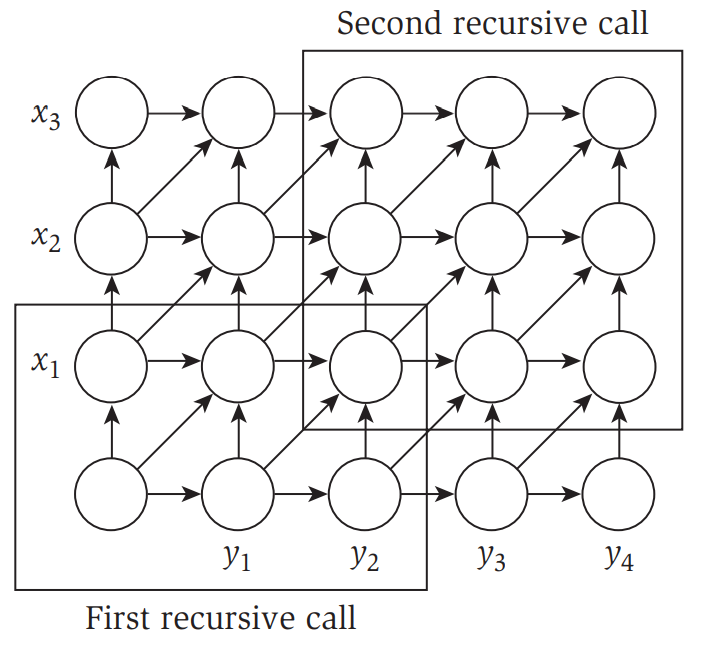
\includegraphics[width=8cm, keepaspectratio]{capitoli/dynamic_programming/imgs/seq_align_recurrence.png}
    \caption{La figura mostra il funzionamento dell'algoritmo appena descritto.}
\end{figure}
